\documentclass[a4paper]{report}

%====================== PACKAGES ======================
\usepackage[utf8]{inputenc}
\usepackage[T1]{fontenc}
\usepackage[french]{babel}
\usepackage{amsmath}
\usepackage[colorinlistoftodos]{todonotes}
\usepackage{url}
\usepackage{multicol}
%Refs
\usepackage{caption}

\usepackage[authoryear]{natbib}


%pour les informations sur un document compilé en PDF et les liens externes / internes
\usepackage{hyperref}
%pour la mise en page des tableaux


\usepackage{enumitem}
\usepackage{float}%pour gérer les positionnement d'images
\usepackage{array}
\usepackage{booktabs}
\usepackage{multirow}
\usepackage{lscape}
\usepackage{amssymb}
\usepackage{pifont}
\usepackage{tabularx}
\usepackage{longtable}
%Images and figures
\usepackage{setspace}
\usepackage{graphicx}
\setcounter{secnumdepth}{3}

\usepackage{hyperref}
\hypersetup{
	colorlinks,
	citecolor=blue,
	filecolor=black,
	linkcolor=black,
	urlcolor=black
}

% for termes
\usepackage{tgtermes}
%pour utiliser \floatbarrier
%\usepackage{placeins}
%\usepackage{floatrow}
%espacement entre les lignes
\usepackage{setspace}

%modifier la mise en page de l'abstract
\usepackage{abstract}
%police et mise en page (marges) du document

%Mis en page :
\usepackage[top=2cm, bottom=2cm, left=2cm, right=2cm]{geometry}
%Footer and Header
\usepackage{fancyhdr}
\setlength{\headheight}{13.1pt}
\pagestyle{fancyplain}
\lhead{}
\cfoot{}
\fancyfoot[R]{\thepage}
\renewcommand{\baselinestretch}{1.5}

%Pour les galerie d'images
\usepackage{subfig}
%Page de garde
\usepackage{framed}


%Abbreviations
\usepackage[french]{nomencl}
\makenomenclature
%Rotating
 \usepackage{rotating}
 \usepackage{tikz}
\newcommand*\rot{\rotatebox{90}}
%\hypersetup{urlcolor=black, colorlinks=bleu}  Colors hyperlinks in blue - change to black if annoyingv`	
%====================== INFORMATION ET REGLES ======================

%rajouter les numérotation pour les \paragraphe et \subparagraphe
\setcounter{secnumdepth}{4}
\setcounter{tocdepth}{4}

\hypersetup{							% Information sur le document
pdfauthor = {KEBAILI Zohra Kaouter,
		KECHIDA Fatima Zahra,
		},			% Auteurs
pdftitle = {Plateforme de test multicritères adapté aux solutions
	multi-biométriques},			% Titre du document
pdfsubject = {Mémoire de Projet},		% Sujet
pdfkeywords = {Tag1, Tag2, Tag3, ...},	% Mots-clefs
pdfstartview={FitH}}					% ajuste la page à la largueur de l'écran
%pdfcreator = {MikTeX},% Logiciel qui a crée le document
%pdfproducer = {}} % Société avec produit le logiciel
%======================== DEBUT DU DOCUMENT ========================
\renewcommand{\baselinestretch}{1.3}
\renewcommand{\thetable}{\Roman{table}}
\captionsetup[table]{name=Tableau}
\begin{document} 
%page de garde
%====================== INCLUSION DES PARTIES ======================

\begin{titlepage}
 \begin{center}
 
\includegraphics[scale=0.9]{Others/Resources/entete.png}\\
 \vspace*{1cm}
  \LARGE
  \textbf{Rapport du module Génie logiciel\\}
  \large
 
  \LARGE
  	\vspace{2cm}
  \textbf{Option: Systèmes et ingénierie de logiciels}\\
  \vspace{1cm}
  \LARGE
  \textbf{Thème}\\
  \vspace{1cm}
  \LARGE
  \setlength{\fboxsep}{0.5cm}
  \begin{framed}
	\textbf{Les anti-patrons linguistiques}
  \end{framed}
  \vspace{2cm}
  \begin{table}[H]
   \setlength{\tabcolsep}{2cm}
    \large
	\centering
	\begin{tabular}{ll}
		\textbf{Réalisé par :}    
		 & \textbf{Encadré par : } \\  \\
		 -\textsc{Mlle Kebaili} Zohra Kaouter 
	
	& -\textsc{ Mme Bousbia} Nabila   \\
	

	\end{tabular}
  \end{table}
  \vspace{\fill}
  \large
  \textbf{Promotion 2017/2018}
        
 \end{center}
\end{titlepage}
\pagenumbering{roman}
\setcounter{page}{2}
\cleardoublepage
\addcontentsline{toc}{chapter}{\contentsname}
\tableofcontents
\cleardoublepage
\addcontentsline{toc}{chapter}{\listfigurename}
\listoffigures
\cleardoublepage
\addcontentsline{toc}{chapter}{\listtablename}
\listoftables
\cleardoublepage
\chapter*{Liste des sigles et abréviations}% Main chapter title
\begin{table}[H]
	\label{my-label}
	\begin{tabular}{ll}
		\textbf{API} & Application Programming Interface    \\
		\textbf{AST}   & Arbre Syntaxique Abstrait                          \\
		\textbf{CBO}  & Coupling Between Objects                \\
		\textbf{IR}  & Information Retrieval                 \\
		\textbf{LOC}  & Ligne Of Code                     \\
		\textbf{LSI}  & Latent Semantic Indexing                    \\
		\textbf{NL}  & Natural Language               \\
		\textbf{OO} & Orienté Objet \\
			\textbf{RESTful} & REpresentational State Transfer \\
			\textbf{SOA} & Architecture Orientée Service \\
			\textbf{SQL} & Structured Query Language \\
		\textbf{SVM} & Machines à Vecteurs de Support                \\
		
		\textbf{SP}   & Singulier Points                        
	\end{tabular}
\end{table}
\pagenumbering{arabic}

\chapter*{Introduction générale}
%\section{Introduction}
\tab Avec le développement logiciel continu et rapide, un programme subit beaucoup de changements pendant son cycle de vie, ce qui engendre des fautes suite à des mauvaises habitudes exercées par les développeurs sous préssion ou par ignorance. Ces mauvaises pratiques affecte la qualité logicielle et rend difficile la compréhesion du code que ce soit par l’auteur du code lui même aprés quelques modifications ou bien par d’autres développeurs lors de la maintenance. Cette derniere avec ses types: Corrective, prenventive, adaptive et  perfective, represente une activité enivitable lors du développement logiciel et vise à produire un logiciel de qualité. \\ \tab

Pour améliorer la qualité logicielle, plusieurs techniques existent, parmi ces techniques: l’utilisation de l’information linguistique, l’utilisation des bons identificateurs, la bonne documentation et l’utilisation du bon lexique. C’est pourquoi, de nouveaux travaux de recherches sont apparus pour exploiter l’information linguistique d’un programme pour identifier les mauvaises pratiques liées au coté linguistique d’un programme ce qui a mené à l’apparition des «anti-patrons linguistiques». \\ \tab

L’objectif de ce rapport est de comprendre ce qu’est un anti-patron linguistique, les anti-patrons linguistiques connus jusqu’à maintenant et comment les détecter.
\pagestyle{fancy}


\newpage
\section{Généralités}
Introduction
Une conception parfaite dès le premier coup n’existe pas, ce qui fait de la tâche de conception une tâche itérative. Les concepteurs avec l’expérience ont remarqué qu’il y a quelques chose qui se répètent d’une conception à l’autre , ce qui a donné naissance à la notion de « patron » et « anti patron » de conception .
\section{Généralités sur les patrons de conception}
Ce terme introduit pour la premiere fois par Koenig en 1998, veut dire les mauvaises solutions reccurentes à des probblèmes de systèmes logiciels\cite{brown1998antipatterns}. Il est important pour les développeurs de connaître les anti-patrons pour savoir les situations où une solution peut avoir un impact négatif et donc l’éviter.
Comme les patrons, les anti-patrons ont leur documentation aussi\cite{arnaoudova2010defining}:
\begin{itemize}
\item \textbf{La pseudo-documentation}: donne le nom et le problème de l’anti-patron en question.
\item \textbf{La mini-documentation}:fournit le nom de l’anti-patron, le problème et la solution proposée.
\item \textbf{la documentation complète}:donne le nom le plus connus,d’autres noms s’il en existe,Frequent niveau: à quel niveau cet anti-patrons peut être détécté: niveau application, micro architecture, framework..etc, nom de la solution et son type, les forces déséquilibrées qui ont été sous-estimées comme la gestion de fonctionnalités ou gestion de complextié, la forme génerale de l’anti-patron donnée sous forme de diagramme, symptomes et conséquences, les exceptions connues où cet anti-patron n’a pas d’impact négatif, d’autres anti-patrons liés à l’anti-patron en question, exemple, applicabilité à d’autres niveaux.
\end{itemize}
\\
Les anti-patrons sont dùs à:
\begin{itemize}
\item  La conception sous des contraintes de temps.
\item  Le changement continu du code.
\item Le non-respect des bonnes pratiques de conception et de codage.
\item l’ignorance et/ou la fiérté des developpeurs.
\end{itemize}
\\

L'ensemble des anti-patrons identifiés ont été catégorisés en\cite{brown1998antipatterns}:
\begin{itemize}
\item Anti patrons de développement.
\item Anti patrons de gestion de projet.
\item Anti patrons d’architecture.

   \end{itemize}
\\
Dans la figure \ref{fig:patanti} ci-dessous, \cite{brown1998antipatterns} illusitre la relation entre les patrons et les anti-patrons que ne verrons juste aprés.
\begin{figure}[H]
	\centering
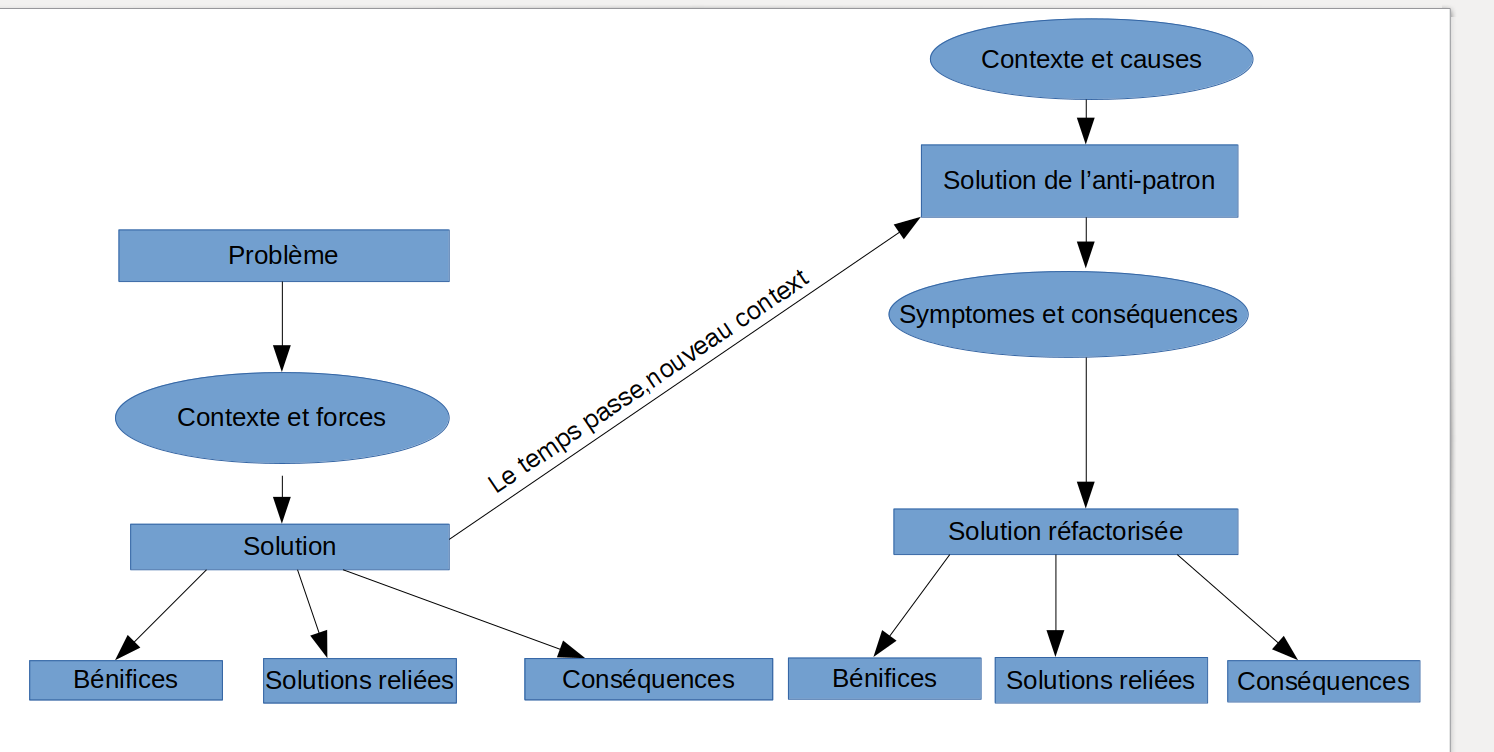
\includegraphics[width=0.9\linewidth]{Others/Resources/patronetantipatron.png}
	\caption{La relation entre les patrons et les anti-patrons \cite{brown1998antipatterns}.}
		\label{fig:patanti}
	\end{figure}
\section{Les anti-Patrons linguistiques}

\label{aplinguistique}
Ils representent une sous-classe des anti-patrons de développement. Ils consistent en les mauvaises habitudes de nomination, de documentation et de choix d’identificateurs  des differentes entités(variables, méthodes, classe-pour les programmes OO...etc) qui reviennent souvent dans les systèmes logiciels qui peuvent affecter la compréhension du code source et/ou la qualité logicielle \cite{brown1998antipatterns}.
L’anti patron linguistique peut etre documenté comme tout autre anti patron, dans ce rapport, nous présentons pour chaque anti-patron linguistique:
\begin{itemize}
\item Son nom
\item Sa description
\item Est ce qu’il concerne une méthode ou un attribut
\item Un exemple tiré d’un vrai programme 
\item Les conséquences possibles de cet anti-patron.
\end{itemize}\\
Puisque nous nous intéressons dans un premier temps, qu’à l’analyse  des attributs et des méthodes dans un code, cette analyse peut être appliquée à d’autres artifacts logiciels comme les diagrammes de classe et les spécifications des APIs.\\

À leurs tours, les anti-patrons linguistiques sont répartis en trois sous-classes à détailler dans le paragraphe suivant pour les méthodes et les attributs \cite{palomba2015anti}:
\begin{itemize}
\item Does more than it says.
\item Says More than it Does
\item Does the Opposite
\end{itemize}
\renewcommand{\thesubsection}{\thesection.\alph{subsection}}
\subsection{Does more than it says}
Ce sont les anti-patrons qui sont détéctés lorsqu’il y a des actions plus que la signature d’une méthode propose \cite{arnaoudova2013new}.

\begin{enumerate}
    

\item \textbf{Plus que des getters} 
\begin{itemize}
\item Description: lorqu’elles fournissent plus que l’attribut concerné en mettant d’autres instructions
\item Appliqué aux: Méthodes
\item Exemple: montré dans la fiqure \ref{fig:un_un} ci-dessous.
	\begin{figure}[H]
	\centering
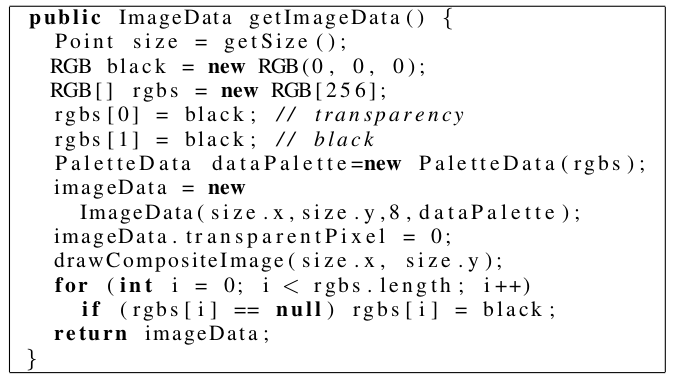
\includegraphics[width=0.9\linewidth]{Others/Resources/un_un.png}
	\caption{Exemple d'un getter qui fait plus que son travail \cite{arnaoudova2013new}.}
		\label{fig:un_un}
	\end{figure}
\item Conséquences: l’utilisation de tels getters engendre l’allocation de nouveaux objets que les getters normallement n’allouent pas.
\end{itemize}
\item \textbf{plus qu’une méthode «is»}
\begin{itemize}
\item Description: Les méthodes qui commencent par “Is” qui sont supposées retourner un booléen mais elles retournent d’autres informations.
\item Appliqué aux: Méthodes
\item Exemple: la figure \ref{fig:un_deux} ilustre un exemple de cet anti-patron.
	\begin{figure}[H]
	\centering
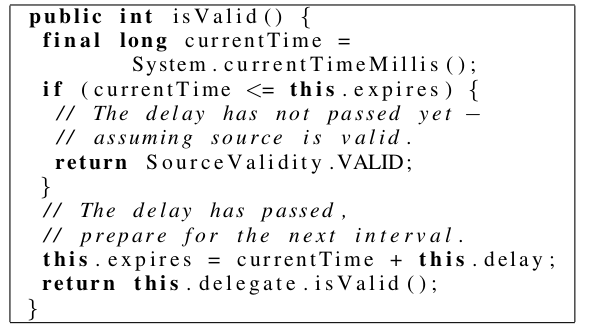
\includegraphics[width=0.9\linewidth]{Others/Resources/un_deux.png}
	\caption{Exemple d'une méthode de type "is" qui fait plus que son travail\cite{arnaoudova2013new}.}
		\label{fig:un_deux}
	\end{figure}
\item Conséquences: une erreur sera déclenchée au moment de la compilation sinon un malentendu de la part des développeurs qui feront la maitenance du programme risque de se produire.
\end{itemize}

\item \textbf{Setter avec retour}
\begin{itemize}

\item Description: Les méthodes setters servent à assigner une valeur à un attribut privé.\\
Ces méthodes ne retournent rien normalement, elles commencent par «set», si un setter se trouve avec une valeur de retour, il doit être renomé.
\item Appliqué aux: Méthodes
\item Exemple: montré dans la figure \ref{fig:un_trois}.
\begin{figure}[H]
	\centering
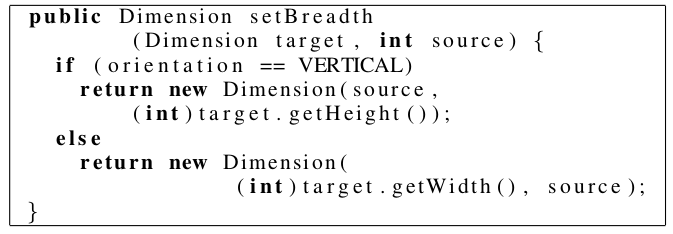
\includegraphics[width=0.9\linewidth]{Others/Resources/un_trois.png}
	\caption{Exemple d'une méthode setter avec retour \cite{arnaoudova2013new}.}
		\label{fig:un_trois}
	\end{figure}
\item Conséquences: il se peut que la méthode setter retourne une valeur liée à un comportement inattendu donc l’erreur ne sera pas captée.

\end{itemize}

\item \textbf{Attendre mais pas recevoir une seule instance}
\begin{itemize}
\item Description: Quand le nom de la méthode fait l’intention de recevoir un seul objet et pas une collection.
Soit une documentation doit être fournie ou bien la méthode doit être renomée.
\item Appliqué aux: Méthodes.
\item Exemple: montré dans la figure \ref{fig:un_quatre}.
\begin{figure}[H]
	\centering

\includegraphics[width=0.9\linewidth]{Others/Resources/un_quatre.png}
	\caption{Exemple de l'anti patron linguistique: Attendre mais pas recevoir une seule instance \cite{arnaoudova2013new}.}
		\label{fig:un_quatre}
	\end{figure}
\item Conséquences: ça ne va pas apparaître au moment de l’execution mais des problèmes de codage pour le développeur, ce dernier va s’attendre à traiter un seul objet, mais il recevra une collection donc, il va être obligé à vériger le corps de la méthode.

\end{itemize}

\end{enumerate}
\subsection{Says More than it Does}
Cet anti-patron apparait lorsqu'une méthode fait mois que ce que la signature d'une méthode propose\cite{arnaoudova2013new}.
\begin{enumerate}
    

\item \textbf {Condition non implémentée}
\begin{itemize}
    \item Description: Quand les commentaires proposent un comportement conditionnel mais le code ne le contient pas.
\item Appliqué aux: Méthodes
\item Exemple: montré dans la figure \ref{fig:deux_un}
\begin{figure}[H]
	\centering
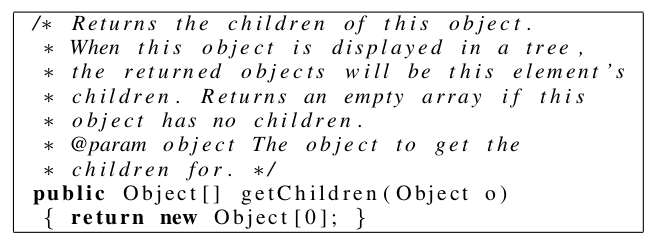
\includegraphics[width=0.9\linewidth]{Others/Resources/deux_un.png}
	\caption{Exemple de l'anti-patron linguistique: Condition non implémentée \cite{{arnaoudova2013new}}.}
		\label{fig:deux_un}
	\end{figure}

\item Conséquences: \\
\begin{enumerate}
    \item La contradiction entre la documentation et le comportement du code va pousser à croire qu’il y a une erreur.
     \item Durant les tests en boite noire, le testeur va inverstir de son temps et effort pour préparer des cas de test selon les differentes conditions mentionnées dans la documentation alors qu’un seul cas pourrait suffir.

\end{enumerate}

\end{itemize}

\item \textbf {Méthode de validation qui ne confirme pas}
\begin{itemize}
\item Description: Une méthode de validation ne retourne pas une valeur pour confirmer cette validation.
\item Appliqué aux: Méthodes
\item Exemple: montré sur la figure \ref{fig:deux_deux}.
\begin{figure}[H]
	\centering
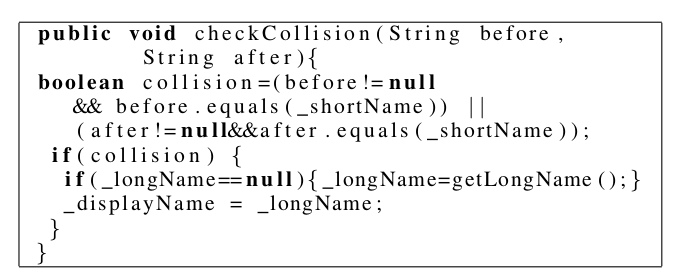
\includegraphics[width=0.9\linewidth]{Others/Resources/deux_deux.png}
	\caption{Exemple d'une méthode de validation qui ne confirme pas\cite{arnaoudova2013new}.}
		\label{fig:deux_deux}
	\end{figure}

\item Conséquences: quelqu’un peut ne pas savoir comment utiliser la sortie de cette méthode, souvent cette sortie est stockée dans une variable quelque part et c’est pas clair au cas d’oubli pour le developpeur ayant écrit cette méthode ou bien au cas de maintenance .
\end{itemize}
\item \textbf{Une méthode getter qui ne retourne rien}
\begin{itemize}
\item Description: le nom de la méthode fait s'attendre à une valeur de retour et ce n’est pas le cas.
\item Appliqué aux: Méthodes.
\item Exemple: montré dans la figure \ref{fig:deux_trois}.
\begin{figure}[H]
	\centering
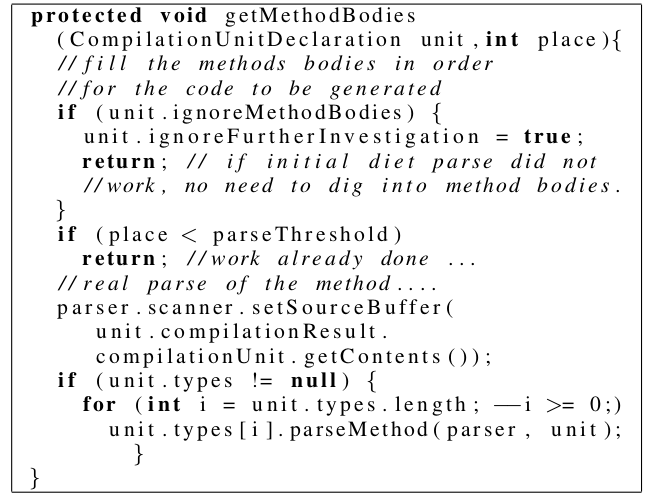
\includegraphics[width=0.9\linewidth]{Others/Resources/deux_trois.png}
	\caption{Exemple d'une méthode getter qui ne retourne rien \cite{arnaoudova2013new}.}
		\label{fig:deux_trois}
	\end{figure}
\item Conséquences: quelqu’un peut assigner la valeur de retour attendue par la méthode getter à une variable et puisque ce n’est pas possible, il va chercher à comprendre le code de la méthode pour trouver la valeur qu’elle fallait retourner.
\end{itemize}

\item \textbf {Question sans réponse}
\begin{itemize}
\item Description: le nom de la méthode commence par «is» ce qui fait s'attendre à un booléen comme valeur retournée mais réellement la méthode ne retourne rien.
\item Appliqué aux: Méthodes.
\item Exemple: montré sur la figure \ref{deux_quatre}.
\begin{figure}[H]
	\centering

\includegraphics[width=0.9\linewidth]{Others/Resources/deux_quatre.png}
	\caption{Exemple d'une méthode question sans réponse\cite{arnaoudova2013new}.}
		\label{fig:deux_quatre}
	\end{figure}
\item Conséquences: Consequences similaires à celle de “une méthode getter qui ne retourne rien". Dans ce cas ,le développeur va s’attendre à ce qu’il peut utiliser la valeur de retour dans le control d’une condition et ce n’est pas possible car elle ne retourne pas un booléen.
\end{itemize}

\item \textbf {Méthode de transformation sans retour}
\begin{itemize}
\item Description: le nom de la méthode donne l’impression qu’elle transforme un objet mais aucune valeur n’est retournée.
\item Appliqué aux: Méthodes.
\item Exemple: donné dans la figure \ref{fig:deux_cinq}.
\begin{figure}[H]
	\centering

\includegraphics[width=0.9\linewidth]{Others/Resources/deux_cinq.png}
	\caption{Exemple d'une méthode de transformation sans retour\cite{arnaoudova2013new}.}
		\label{fig:deux_cinq}
	\end{figure}
\item Conséquences: Similaire aux précedantes. Ici la valeur de retour pourrait être assignée à une variable dont le nom est inspiré du nom de la méthode.
\end{itemize}

\item \textbf{Attendre une collection mais ne pas la recevoir}
\begin{itemize}
\item Description: Une collection est retournée au lieu d’un seul objet.
\item Appliqué aux: Méthodes.
\item Exemple: montré dans la figure \ref{fig:deux_six}.
\begin{figure}[H]
	\centering

\includegraphics[width=0.9\linewidth]{Others/Resources/deux_six.png}
	\caption{Exemple de l'anti-patrons: Attendre une collection mais ne pas la recevoir\cite{arnaoudova2013new}.}
		\label{fig:deux_six}
	\end{figure}
\item Conséquences: un developpeur peut s’attendre à une collection d’objet et donc il peut utiliser des patrons qui manipulent des collections comme iterator.
\end{itemize}
\end{enumerate}
\subsection{Does the Opposite}
Cet anti-patron apparait dans le cas où il y a une relation d'opposition quelque part dans une méthode\cite{arnaoudova2013new}.
\begin{enumerate}
    

\item \textbf {Le nom de la méthode et le type de retour sont opposés}
\begin{itemize}
\item Description: Ce que veut le nom de la méthode est contradictoire au type de la valeur retournée.
\item Appliqué aux : méthodes.
\item Exemple:montré dans la figure \ref{fig:trois_un}.
\begin{figure}[H]
	\centering
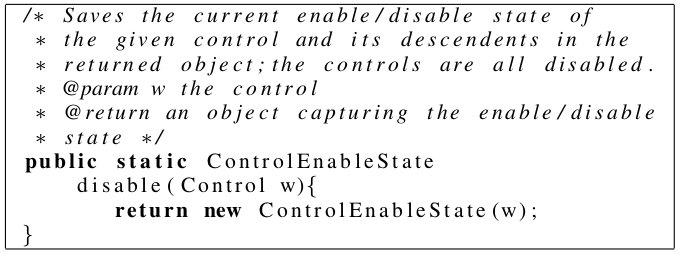
\includegraphics[width=0.9\linewidth]{Others/Resources/trois_un.png}
	\caption{Exemple de l'anti-patrons: Le nom de la méthode et le type de retour sont opposés\cite{arnaoudova2013new}.}
		\label{fig:trois_un}
	\end{figure}
\item Conséquences: les développeurs peuvent se tromper par rapport à la valeur retournée, ça peut ne pas avoir un impact si la méthode retourne un booléen.
\end{itemize}

\item \textbf {La signature de la méthode et les commentaires sont opposés}
\begin{itemize}
\item Description: La documentation de la méthode est contradictoire à sa déclaration(son nom ou bien type retourné).

\item Appliqué aux: Méthodes.
\item Exemple: montré dans la figure \ref{fig:trois_deux}.
\begin{figure}[H]
	\centering
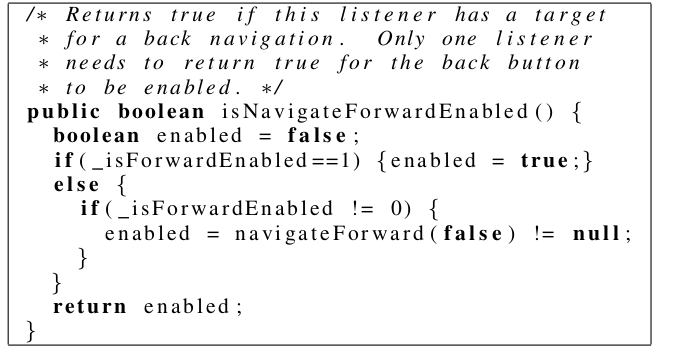
\includegraphics[width=0.9\linewidth]{Others/Resources/trois_deux.png}
	\caption{Exemple de l'anti-patrons:  Signature de la méthode et les commentaires sont opposés\cite{arnaoudova2013new}.}
		\label{fig:trois_deux}
	\end{figure}
\item Conséquences: similaires aux précedantes et peuvent être plus grave car le développeur sera confus, est ce qu’il doit suivre les commentaires ou bien la signature de la méthode, l’un des deux doit étre mis à jour.
\end{itemize}
\end{enumerate}
\subsection{Contains more that it says}
Ce type d'anti-patron concerne les  attributs signifiont plus qu'ils sont réellement \cite{arnaoudova2013new}.
\begin{enumerate}
    

\item \textbf {Dit une chose mais contient beaucoup de choses}
\begin{itemize}
\item Description: Un attribut dont le nom signifie qu’il contient une seule instance mais son type stoque une collection d’objets.
\item Appliqué aux: Attributs.
\item Exemple: montré dans la figure\ref{fig:quatre_un}.
\begin{figure}[H]
	\centering

\includegraphics[width=0.9\linewidth]{Others/Resources/quatre_un.png}
	\caption{Exemple de l'anti-patrons:  Dit une chose mais contient beaucoup de choses\cite{arnaoudova2013new}.}
		\label{fig:quatre_un}
	\end{figure}
\item Conséquences: manque de compréhension de la classe, quand cet attribut change on peut pas savoir l’impact du changement sur les objets manipulés
\end{itemize}

\item \textbf {Nom de booléen mais le type non booléen}
\begin{itemize}

\item Description: Un attribut qui donne l’impression qu’il a deux valeurs soit vraie ou fausse mais sa déclaration est de type  autre que booléen.
\item Appliqué aux: Attributs.
\item Exemple:  comme l’illustre la figure \ref{fig:quatre_deux}
\begin{figure}[H]
	\centering
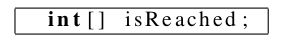
\includegraphics[width=0.9\linewidth]{Others/Resources/quatre_deux.png}
	\caption{Exemple de l'anti-patrons: Nom de booléen mais le type non booléen\cite{arnaoudova2013new}.}
		\label{fig:quatre_deux}
	\end{figure}
\item Conséquence:Le développeur s’attend à ce qu’il soit capable d’utiliser cet attribut dans une instruction de condition mais le type déclaré ne le permet pas .

\end{itemize}
\end{enumerate}
\subsection{Says more than it contains}
Ce type d'anti-patron concerne les  attributs signifiont moins qu'ils sont réellement\cite{arnaoudova2013new}.
\begin{enumerate}
    
\item \textbf {Dit beaucoup de choses mais contient une seule}
\begin{itemize}
\item Description: Un attribut qui donne l’impression du’il contient une collection d’objet mais en réalité il contient un seul objet.
\item Appliqué aux: Attributs.
\item Exemple: montré dans la figure \ref{fig:cinq}
\begin{figure}[H]
	\centering

\includegraphics[width=0.9\linewidth]{Others/Resources/cinq.png}
	\caption{Exemple de l'anti-patrons: Dit beaucoup de choses mais contient une seule\cite{arnaoudova2013new}.}
		\label{fig:cinq}
	\end{figure}
\item Conséquences:manque de compréhesion de l’impact du changement de la l’attribut.
\end{itemize}
\end{enumerate}
\subsection{Contains the opposite}
Ce type d'anti-patron apparait s'il y a une contradition entre un attribut et les commentaires \cite{arnaoudova2013new}.
\begin{enumerate}
    

\item \textbf{L’attribut et son type sont opposés}
\begin{itemize}
\item Appliqué aux: Attributs.
\item Exémple: montré sur la figure \ref{fig:six_un}
\begin{figure}[H]
	\centering
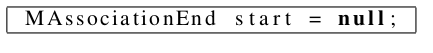
\includegraphics[width=0.9\linewidth]{Others/Resources/six_un.png}
	\caption{Exemple de l'anti-patrons: L’attribut et son type sont opposés\cite{arnaoudova2013new}.}
		\label{fig:six_un}
	\end{figure}
\item Conséquences: ça peut mener à des malentendus, par exemple
un booléen contient l’information qui peut être directlement utilisée dans une condition mais on risque d’inverser les blocs de si sinon.
\end{itemize}
\item \textbf{La signature de l’attribut et le commentaire sont opposés}
\begin{itemize}
\item Description: La docmentation de l’attribut peut être contradictoire au nom ou type de cet attribut.
\item Appliqué aux: Attributs
\item Exemple: montré dans la figure \ref{fig:six_deux}
\begin{figure}[H]
	\centering
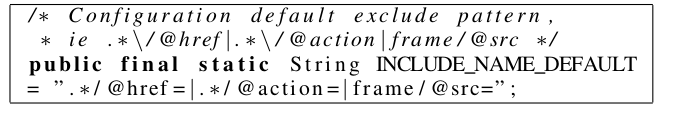
\includegraphics[width=0.9\linewidth]{Others/Resources/six_deux.png}
	\caption{Exemple de l'anti-patrons: La signature de l’attribt et le commentaire sont opposés\cite{arnaoudova2013new}.}
		\label{fig:six_deux}
	\end{figure}
\tem Conséquences: sans analyser profédemment le code source,le developpeur peut ne pas comprendre le rôle de l’attribut.
\end{itemize}

\end{enumerate}


\section{La détéction des anti-patrons linguistiques}
toute détéction d’anti-patron doit passer par deux étapes\cite{brown1998antipatterns}:
\begin{itemize}
    

\item Extraire les informations du code source pour identifier les symptomes des mauvais choix
\item Définir les bons algorithmes pour savoir les anti-patrons linguistques correspondants aux symptomes extraites.
\end{itemize}
\textbf{Pourquoi est-il important de détecter les anti-patrons linguistiques?}\\
Les identificateurs mal choisis augmentent l’effort de comprésension du code source, ces identificateurs peuvent être des mots du dictionnaire, acronyme, ou de simples chaines de caracteres.
L’utilisation des termes identiques dans differents contextes peut augmeter le risque d’apparition de fautes. Cette information prouvée en utilisant deux métriques:l’entropie d’un terme et la couverture d’un contexte par un terme,le but est de montrer que le choix de certains termes augmente la prédisposition aux fautes.Deux métriques sont exploitées à ce niveaux:
\begin{itemize}
    

\item L’entropie d'un terme:  mesure la dispersion physique qui est  le degrés auquel un terme est éparpillé à travers les identificateurs des differentes entités\cite{arnaoudova2010defining}.
\item La couverture d’un context: mesure la dispersion conceptuelle qui est la relation entre ces entités\cite{arnaoudova2010defining}.
\end{itemize}
Si ces deux mesures sont élevées ça veut dire que les termes qui sont beaucoup éparpillés dans le programme  sont utilisés dans des entités non reliées l’une à l’autre  ce qui augmente le risque de prédisposition aux fautes.\\

La détéction des anti-patrons linguistiques est reliée à des domaines\cite{arnaoudova2016linguistic}:
\begin{enumerate}


\item L’entropie et les métriques basées sur la récupération de l’information (information retrieval -based metrics):\\ Plusieurs métriques basées sur l’entropie existent, elles peuvent être appliquées pour expliquer les changements qu’une classe subit à travers plusieurs versions, utilisées pour expliquer la cohesion d’un composant, les méthodes de  la récupération de l’information sont utilisées aussi pour mesurer la qualité d’un code , par exemple, elle servent à mesurer la complexité d’un programme orienté objet, les SVMs et Latent Semantic Indexing(LSI) sont utilisés pour mesurer la cohesion d’une classe, les SVMs sont appliqués pour extraire les identificateurs des entités d’un part, et les identificateurs des commentaires, comparer entre eux, la similarité entre eux indique des entités de bonne qualité.
\item Métriques et prédisposition aux fautes:\\
Ce sont les recherches qui ont pour but de trouver les bonnes métriques comme LOC et CBO qui prédictent le mieux les fautes en calculant la correlation entre ces métriques et la prédisposition aux fautes.
\item L’information linguistique d’un code source:\\
Concerne les recherches de langues essentiellement comme l’ambiguité lexicale, le refactoring stratégique des identificateurs du code source basé sur le lexique standard, d’autres recherches dans ce domaine ont montré que les programmes commentés sont mieux compris par rapportt aux programmes non commentés,les programmes contenant des identificateurs à mots complets sont mieux compris par rapport aux programmes qui contiennent des identificateurs à mots incomplets.
\item Traitement du langage naturel:\\
Ce domaine s’interessent à trouver et mesurer les differents types d’ambiguité(lexicale, syntaxique…) dans le langage naturel, à cause de cette ambiguité, une expression peut être comprise de deux maniere differentes.
\end{enumerate}
\\
\newline
Dans le paragraphe suivant, nous détaillons la détection des anti-patrons linguistiques citées dans la section \ref{aplinguistique}\cite{arnaoudova2016linguistic}:\\
\renewcommand{\thesubsection}{\thesection.\alph{subsection}}
\subsection{Détection des anti-patrons linguistiques de type "Does more than it says"}
\begin{enumerate}
    

\item \textbf{Plus que des getters}\\
Trouver les getters, qui sont les méthodes qui commencent par « get » et se terminent par une chaine de caractères qui correspond à un attribut de meme classe,le type de cet attribut et le type de la valeur retournée par le getter doivent etre les memes. Ensuite,identifier les getters qui fournissent des actions autres que retourner une valeur d’attribut. Des cas où l’attribut est mis à jour avant qu’il soit retourné ne sont pas pris en compte, comme le patron proxy et singleton.
Pour une détection basée sur les expressions du sommet de l’arbre syntaxique abstrait( AST)  autres que l’intruction return est permise sauf dans le cas où un fils d’un control de condition pour la valeur nulle. Autres mesures de complexité comme LOC  ou la compléxité cyclomatique de McCabe peuvent etre utilisés pour une détection simple mais moins exacte.
\item \textbf{plus qu’une méthode «is»}\\
Trouver les méthodes qui commencent par «is» dont le type de retour 
\item \textbf{Setter avec retour}\\
Trouver les méthodes qui commencent par « set » dont le type de retour est different de void.
\item \textbf{Attendre mais pas recevoir une seule instance}\\
Trouver les méthodes qui retournent une collection ( vecteur,tableau…) dont le nom se terminent par un nom en singulier et qui ne contient pas un mot qui signifie une collection.
\end{enumerate}
\subsection{Détection des anti-patrons linguistiques de type "Says More than it Does"}
\begin{enumerate}
\item \textbf{Condition non implémentée}\\
Trouver les méthodes contenant au moins une phrase conditionnelle dans les commentaires, sans qu’il y a des intructions de conditions dans le code.
\item \textbf{Méthode de validation qui ne confirme pas}\\
Trouver les méthodes de validation dont le nom commence par « validate »,check, ensure...etc où le type de retour est void ,sans qu’il y a les instructions d’exception.
\item \textbf{Une méthode getter qui ne retourne rien}\\
Trouver les méthodes dont le nom donne l’impression qu’il y a une valeur de retour mais dont le type de retour est void.
\item \textbf {Question sans réponse}\\
Trouver les méthodes dont le nom commencent par : is ou has, ie, il donne l’impression d’une question,mais le type de retour est void.
\item \textbf{Méthode de transformation sans retour}\\
Trouver les méthode dont le nom propose une transformation, exemple : toString,list2array...etc mais le type de retour est void.
\item \textbf{Attendre une collection mais ne pas la recevoir}\\
Trouver les méthodes don le nom  donne l’impression qu ‘elle retourne un collection,par exemple, qui commence par «get», «return»…,mais le type de retour n’est pas une collection.
\end{enumerate}

\subsection{Détection des anti-patrons linguistiques de type "Does the Opposite"}
\begin{enumerate}
\item \textbf{Le nom de la méthode et le type de retour sont opposés}\\
Trouver les méthodes dont le nom et le type de retour sont des acronoymes.
 \iextbf{La signature de la méthode et les commentaires sont opposé}\\
Trouver les méthode dont le nom ou le type de retour possede une relation d’acronyme avec son commentaire.
\end{enumerate}
\subsection{Détection des anti-patrons linguistiques de type "Contains more that it says"}
\begin{enumerate}
    \item \textbf{Dit une chose mais contient beaucoup de choses}\\
    Trouver les attributs dont le nom se terminent par un nom singulier mais il est déclaré de type collection.
\item \textbf{Nom de booléen mais le type non booléen}\\
Trouver les attributs dont le nom  commence par  un verbe conjugué au troisieme pronom personnel « is » où « has » par exemple, ou qui se termine par un gérondif mais il est déclaré de type autre que booléen.
\end{enumerate}
\subsection{Détection des anti-patrons linguistiques de type "Says more than it contains"}
\begin{enumerate}
    

\item \textbf{Dit beaucoup de choses mais contient une seule}\\
trouver les attributs contenant un nom au pluriel mais déclaré de type autre que collection.
\subsection{Détection des anti-patrons linguistiques de type "Contains the opposite"}
\end{enumerate}
\begin{enumerate}
    

\item \textbf{L'attribut et son type sont opposés}\\
Trouver les attributs dont le nom et leur type de déclaration sont opposés.
\item \textbf{ La signature de l’attribt et le commentaire sont opposés}
\\Trouver les attributs dont le nom ou bien le type de déclaration possède une relation d’acronyme avec son commentaire.
\end{enumerate}

\section{Implementation d’un outil de  détection des anti-patrons linguistiques}
Pour implémenter un outil de détection automatiques des anti-patrons linguistiques, on procède par des étapes qui sont\cite{arnaoudova2013new}:\\
\begin{enumerate}
    

\item \textbf {Exraction des faits à partir du code source}: En utilisant un outil analyseur(parser) comme srcml tool on génére un arabre d’analyse à l’aide duquel on collecte les elements utiles comme les attributs, les noms des méthodes, les commentaires, la pésence des exceptions et des conditions
\item \textbf {Analyse des identificateurs et des commentaires}:
Cette étape a pour but d’identifier les termes qui composent les identificateurs,d’abord en applicant les heuristiques «camel case» et «under score» pour avoir les termes, puis en utilisant l’analyseur de Stanford pour le langage naturel pour savoir si un terme est un nom , adjective ou adverbe...etc,savoir si un nom est au singulier ou au pluriel, la relation entre les mots comme la négation.
\item \textbf{Lier entre les termes des identificateurs et les termes des commentaires}: En utilisant l’outil WordNet ontology, des liaisons de synonymes ou  d’acronymes sont établies.
\end{enumerate}

\section{Les anti-patrons dans les APIs RESTful}
L’architecture SOA est devenue une parmi les plus architecutre adoptées,surtout son style architectural «REpresentational State Transfer» privilégié par beaucoup d’entreprises de production de logiciels comme twitter, facebook et youtube.
Vu que les developpeurs utilisant ces APIs ont besoins de les comprendre pour pouvoir les exploiter dans leurs applications web, c’est pourquoi, les developpeurs tendent vers chercher les APIs dont les URIs (Uniform Resource Identifiers) sont bien conçus et bien \textbf{nommés}.

Les cinq anti-patrons linguistiques  apparus dans les applications REST \cite{palma2015restful}:
\begin{enumerate}
    

\item \textbf{Noms de ressources contextualisés Vs Noms de ressources non-contextualisés}
\begin{itemize}
    

\item {Description}: l’URI doit être contextuel,ie, les nœuds d’une URI doivent etre sémantiquement reliés au même contexte.Cet anti-patron apparaît si les nœuds d’une URI n’appartient pas sémantiquement au même contexte.
\item Exemple: \\
https://www.example.com/newspapers/players?id=123  est faux mais \\
https://www.example.com/newspapers/media/page?id=123 est correct.
\item Conséquences:\\
Les noms des ressources non-contextualisés ne fournissent pas un contexte clair pour les requêtes qui dégrade la compréhension des URIs de la part des développeurs qui les utilisent.
\end{itemize}

\item \textbf{Noeuds hiérarchiques vs nœuds non-hiérarchiques}
\begin{itemize}
    

\item Description: chaque nœud composant d’une URI doit être hiérarchiquement relié aux nœuds voisins, donc cet anti-patrons apparaît si on trouve des nœuds dans une URI qui ne sont pas hiérarchiquement reliés  à leurs nœuds voisins.
\item Exemple:\\
https://www.example.com/professors/university/faculty/ est faux mais\\ https://www.example.com/university/faculty/professors/ est correct.
\item Conséquences: ça peur induire à une confusion à propos de l’utilité de l’URI et donc son utilisabilité.
\end{itemize}
\item \textbf{URI propre vs URI amorphe}
\begin{itemize}
    

\item Description: Une URI propre est une URI lisible,dont les noms sont minuscules, sans underscore, sans extensions et sans aucun symbole pouvant compliquer la lecture de l’URI sinon cet anti-patron est identifié.
\item Exemple:\\
https://w\itemww.example.com/NEW Customer/ photo01.jpg/ est faux mais \\
https://www.example.com/customers/1234 est correct.
\item Conséquences: Les mots en lettres majuscules et en lettres minuscules ne signifient pas la même ressource,et en général ça peut mener vers une ambguité dans l'écriture de la requête.
\end{itemize}
\item \textbf{URI sans verbes vs une URI CRUDy}
\begin{itemize}
    

\item Description: Cet anti-patrons apparaît si les méthodes HTTPs : GET, PUT, POST,DELETE sont utilisés dans des URIs contenant des verbes comme create, update..etc
\item exemple:\\
POST https://www.example.com/update/players/age?id=123 est faux\\
mais POST https://www.example.com/players/age?id=123 est correct.
\item Conséquences:
Cet anti-patron cause une confusion, l’utilisateur d’une API risque de surcharger les méthodes http existantes.
\end{itemize}
\item \textbf{Noeuds singularisés vs Noeuds pluralisés}
\begin{itemize}
    

\item Description: Cet anti-patron apparaît si dans les requêtes put/delete, le dernier est au pluriel ou si dans les requêtes post le dernier nœud est au singulier
\item Exemple:\\
DELETE https://www.example.com/team/players \\
 POST https://www.example.com/team/player sont faux mais \\
DELETE https://www.example.com/team/player \\
 POST https://www.example.com/team/players sont corrects.
\item Conséquences:
Si un nœud pluriel est utilisé à la fin d’une URI de requête PUT/DELETE, le client de l’API ne peut pas créer/supprimer une colection de ressources qui peut causer la reponse serveur « 403 forbidden » et même si la reponse est filtrée,le client de l’API peut tomber dans la confusion entre est ce que le contenu accessible/supprimé est une ressource ou plusieurs ressources.
\end{itemize}
\end{enumerate}
La figure ci-dessous \ref{fig:algocontextualise} illustre l’algorithme de détection de l’anti-patrons « noms de ressources non-contextualisé» dans les applications RESTful \cite{palma2015restful}:
\begin{figure}[H]
	\centering
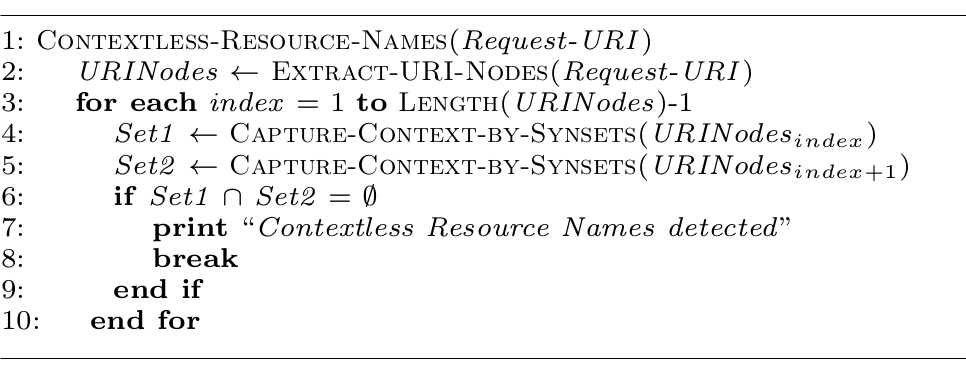
\includegraphics[width=0.9\linewidth]{Others/Resources/algocontextualis.png}
	\caption{L'algorithme de détection de l'anti-patron linguistique noms de ressources non contextualisés \cite{{arnaoudova2013new}}.}
		\label{fig:algocontextualise}
	\end{figure}

L’algorithme procède comme suit :
\begin{itemize}
\item On compare chaque pair de nœud dans une URI 
\item Si on trouve au moins une relation de non-contextualisation
\item Alors l’anti-patron de nom de ressources non-contextualisé.
\end{itemize}
L’ontology WordNet et Stanford CoreNLP pour capter les contextes et effectuer l’analyse sémantique \cite{palma2015restful}.
\\
\cite{palma2015restful} implémentent une solution qui s'appelle "DOLAR"(voir la figure \ref{dolar}) qui détecte les anti-patrons linguistiques dans les applications RESTful, l'article contient les détails de l'implémentation aisni que les résultats de ses tests.
\begin{figure}[H]
	\centering
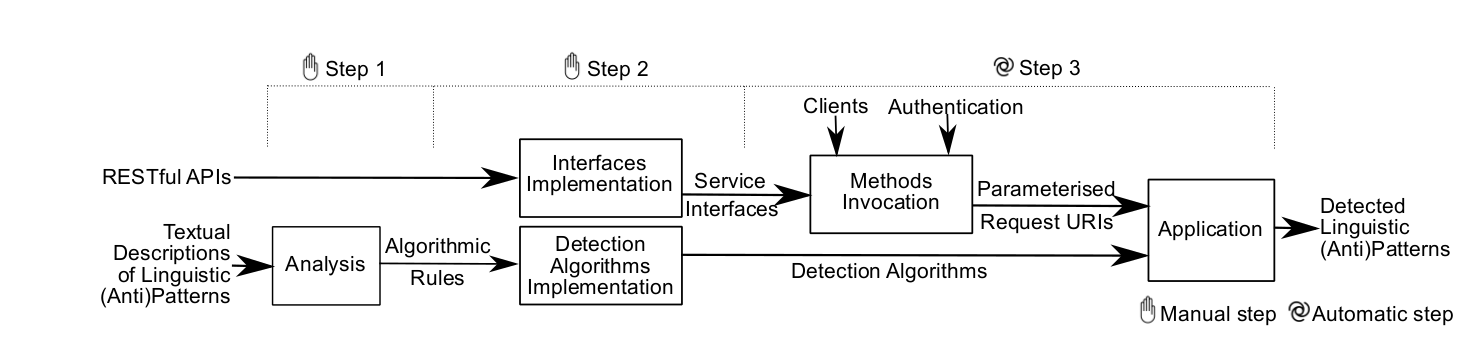
\includegraphics[width=0.9\linewidth]{Others/Resources/dolarapproach.png}
	\caption{L'approche DOLAR \cite{{arnaoudova2013new}}.}
		\label{fig:dolar}
	\end{figure}
\newpage
\section{Conclusion}
\tab Dans ce rapport, nous avons abordé le sujet des anti-patrons linguistiques comme axe de recherches récent dans le domaine de la détection des patrons et des anti-patrons en général. \\ \tab

Cet axe n’est pas encore bien exploité, chose observée pendant la recherches bibliographique, les informations linguistiques ne sont pas toutes exploitées et  peu sont les algorithmes de détection, par exemple l'article \cite{karwin2010sql} propose quelques anti-patrons pour le langage SQL mais les anti-patrons linguistiques SQL ne sont pas invoqués.
\\


\tab Comme synthèse, nous avons établi la liaison entres l’information linguistique,et ses differents métriques et un bon code source,nous avons aussi  touché à l’importance de détéction des anti-patrons linguistiques et leurs solutions refactorisées pour améliorer la qualité logicielle. Il  reste à réaliser un outil pour la détection automatique et exacte des anti-patrons linguistiques avec la possibilité de correction et de refactoring automatique.

\chapter{Système biométrique basé sur l'empreinte digitale}
\label{Chapter2} % Change X to a consecutive number; for referencing this chapter elsewhere, use \ref{ChapterX}

\section{Introduction}
Parmi les nombreuses modalités biométriques existantes, les empreintes digitales (appelée aussi « dermatoglyphe ») sont la plus utilisée pour la reconnaissance des personnes grâce à son unicité, son universalité, aisance de son acquisition et sa permanence \citep{maltoni2009handbook}.\\
Dans ce chapitre, nous présentons les caractéristiques d'empreinte digitale, nous détaillons les différentes étapes de son processus de reconnaissance et nous présentons une variété de méthodes utilisées dans chaque étape.
\section{Caractéristiques des empreintes digitales}

L'empreinte digitale se compose de motifs dessinés par les crêtes et les vallées de la peau. Les caractéristiques liées à l'empreinte digitale sont généralement catégorisées en trois niveaux \citep{hasan2013fingerprint} :
\begin{enumerate}
	
	\noindent\begin{minipage}{0.7\textwidth}% adapt widths of minipages to your needs
		\item 	\textbf{Les détails de niveau 1: }les caractéristiques globales (les points singuliers) visibles à l'œil, il en existe deux types : les points cores (un core est de lieu de courbure maximale des lignes d'empreinte les plus internes), et les deltas (un delta est le lieu de divergence des lignes les plus internes. En d'autres termes un delta est proche du lieu où se séparent deux lignes), et sont considérés comme le centre de l'empreinte digitale, c'est-à-dire celui qui est utilisé pour l'alignement des empreintes digitales lors de la phase d'appariement (voir figure \ref{fig:chapitre2fingerprintlevel1}).   
		
	\end{minipage}%
	\hfill%
	\begin{minipage}{0.3\textwidth}\raggedleft
	 
		\begin{center}
			\begin{figure}[H]
				\centering
				\includegraphics[width=0.50\linewidth]{fingerlevel1}
				\captionsetup{justification=centering}
				\caption{Les points singuliers d'empreintes digitales.}
				\label{fig:chapitre2fingerprintlevel1}
			\end{figure}
		\end{center}
		
	\end{minipage}%
	\item \textbf{Les détails de niveau 2 : }sont les minuties (caractéristiques locales) composées de fins de ligne (terminaisons), bifurcations, lacs, îlots. Elles sont utilisées par la plupart des systèmes automatisés de reconnaissance et peuvent être extraites de manière fiable à partir des images d'empreintes digitales avec une faible résolution (~ 500 dpi (dot per inch = pixels par pouce)) qui est également la résolution standard adoptée par le Federal Bureau d'Investigation (FBI) dans leurs systèmes automatiques d'identification (AFIS) \citep{jain2007pores}.
	
	
	\item \textbf{Les détails de niveau 3 :} sont la forme des bords de crêtes, les crêtes immatures, le contour des arêtes, etc. ce niveau est peu utilisé par les systèmes de reconnaissance, car les images capturées pour extraire les détails de ce niveau sont de haute résolution (1 000 (dpi)) (voir figure \ref{fig:chapitre2fingerprintlevel3}). 
	
	\begin{center}
		\begin{figure}[H]
			\centering
			\includegraphics[width=0.56\linewidth]{fingerlevel3}
			\caption{Les caractéristiques visibles dans le niveau 3.}
			\label{fig:chapitre2fingerprintlevel3}
		\end{figure}
	\end{center}
\end{enumerate}

Le processus de la reconnaissance des empreintes digitales passe par plusieurs phases, la première phase est l'acquisition d'images d'empreintes de l'utilisateur, ensuite un prétraitement des images est faites acquises afin d'améliorer leur qualité est suivi par une extraction de données utiles, et enfin après une comparaison entre le modèle de l'utilisateur et le modèle enrôlé une décision est prise. Et pour réduire le nombre de comparaison d'une empreinte digitale avec les empreintes digitales stockées dans une grande base de données, les images doivent être classifiées en suivant des méthodes de classification.
Il existe trois types d'approches des systèmes de reconnaissance : approches basées sur la corrélation, approches basées sur les minuties et approches basées sur les textures. 
Les approches basées sur les minuties sont les plus utilisés par les systèmes biométriques \citep{jiang2000fingerprint} car elles donnent des résultats plus précises \citep{o1998overview}, et ce sont les approches auxquelles nous nous intéressons le plus dans notre travail. 

\section{Extraction des minuties}
Une fois toutes les étapes de pré-traitement (voir annexe \ref{pretrait}) sont appliquées et l'image binarisée squelettisée de l'empreinte digitale est obtenue, nous extrayons les minuties \citep{tisse2001systeme}. Il y en a deux types de méthodes d'extraction des minuties : les méthodes basées sur la binarisation (avec ou sans squelettisation) et les méthodes directes. Cependant, les méthodes basées sur la binarisation avec une étape de squelettisation qui améliore la qualité de l'image de l'empreinte sont plus utilisées \citep{bansal2011minutiae}, nous les présentons dans ce qui suit :
 \subsection{Extraction avec le nombre de connexions (CN)}
  La plupart de recherches sur la reconnaissance des empreintes digitales extraient les minuties à l'aide de la méthode du nombre de connexions CN (Crossing Number) , comme dans \citep{Thai2003} notamment dans \citep{amengual1997real} , \citep{mehtre1993fingerprint} et \citep{kasaei1997fingerprint}.
\\
Le nombre CN d'un pixel P dans une image binarisée est calculé comme suit \citep{maltoni2009handbook} :
\begin{center}
	\begin{equation}\label{eq:cn}
	CN (P) = \frac{1}{2}\sum_{i=1}^{8}|val (P_{i mod 8 } )-  val(P_{i-1}) |
	\end{equation}
\end{center}
$ P_{i} $ est la valeur du pixel voisin à celui pour qui le CN est calculé.
\\En utilisant les propriétés du CN, chaque pixel d'une crête peut être classé comme un point intermédiaire (non-minutie), une terminaison ou une bifurcation.

\begin{center}
	\begin{figure}[H]
		\centering
		\includegraphics[width=0.6\linewidth]{cn}
		\caption{Nombre de connexions ; a). Point intermédiaire b). Terminaison ; c). Bifurcation \citep{maltoni2009handbook}.}
		\label{fig:chapitre2cn}
	\end{figure}
\end{center}

\subsection{Extraction à base morphologique}
Ces techniques d'extraction sont basées sur une morphologie mathématique dans laquelle l'image est pré-traitée (les étapes de pré-traitement sont expliquées dans l'annexe \ref{pretrait}) et ensuite un autre traitement avec des opérateurs morphologiques (Ouverture) et (Fermeture) est effectué, où l'opération d'ouverture est pour la suppression des pics introduits par le bruit de fond et l'opération de fermeture pour élimination de petites cavités, et enfin, les minuties sont extraites à l'aide de la transformation morphologique en tout ou rien « hit or miss transformation », la technique développe une structure pour chaque type de minutie, par exemple les terminaisons de crête sont les pixels d'une image qui n'ont qu'un voisin dans un voisinage de $ 3 \times 3 $. des exemples d'utilisation de cette technique dans \citep{humbe2007mathematical} et \citep{bansal2010effective}.
\\ Dans certaines méthodes d'extraction, nous procédons par une étape d'élimination des fausses minuties que nous présenterons dans l'annexe \ref{posttrait}.
\section{Appariement}
L'appariement des empreintes digitales est une étape cruciale dans les problèmes d'authentification et d'identification qui consiste à comparer entre deux empreintes digitales et retourne un degré de similarité(un nombre réel appartient à un intervalle) ou décision binaire  (accepté ou non-accepté).
\\
\subsection{Formulation du problème}
Nous représentons dans ce qui suit le modèle enrôlé d'une empreinte digitale par $ (T) $ et le modèle en entrée par$  (E) $. Et chaque élément du vecteur de caractéristiques (vecteur de minuties) en sortie de par $ (M) $, où chaque élément est désigné par : son type (Terminaison ou Bifurcation), ses coordonnées cartésiennes $ (x, y)  $et son orientation($\theta$)(voir Figure \ref{fig:chapitre2minutiarepresentation}). 
\begin{center}
	\begin{equation}\label{eq:t}
	\abovedisplayskip
	\belowdisplayskip
	T=(M_{1},M_{2}, ..., M_{n})\qquad M_{i}=(x_{i},y_{i},\theta_{i})\quad i = 1 .. n
	\end{equation}
\end{center}
\begin{center}
	\begin{equation}\label{eq:e}
	E=(M\prime_{1},M\prime_{2}, ..., M\prime_{n\prime})\qquad M\prime _{i\prime }=(x\prime _{j },y\prime_{j},\theta\prime_{j}) \quad j = 1 .. n\prime
	\end{equation}
\end{center}


\begin{center}
	\begin{figure}[H]
		\centering
		\includegraphics[width=1\linewidth]{minutiarepresentation}
		\captionsetup{justification=centering}
		\caption{Représentation basique des minuties a) une terminaison, b) une bifurcation \citep{maltoni2009handbook}.}
		\label{fig:chapitre2minutiarepresentation}
	\end{figure}
\end{center}
Une minutie $ M_{j} $ dans $  T $ et une minutie $  M_{i} $ dans $ E $ sont considérées appariées, si $ M_{j} $  tombe dans la zone de tolérance de $ M_{i} $ , une zone de tolérance qui définie par  une distance spatiale ($ sd $) maximale et une différence directionnelle ($ dd $) permet de compenser les erreurs inévitables faites lors de la phase d'extraction des minuties ou par les changements de positionnement produits par des distorsions dans l'empreinte digitale (voir les équations \ref{eq:sd} et \ref{eq:dd}). Pour maximiser le nombre de minuties de $ E $ qui correspondent à $ T $ le modèle enrôlé, il faut aligner les deux modèles (cela inclut également le déplacement, la rotation et d'autres transformations géométriques), après l'alignement, un score de similarité pour les deux modèles est calculé en utilisant une fonction d'appariement.

\begin{center}
	\begin{equation}	
	\label{eq:sd}	
	sd(M_{i},M\prime_{j})=\sqrt{(x_{i}-x\prime _{j})^{2}+(y_{i}-y\prime _{j})^{2}} \; \leq r_{0}
	\end{equation}
\end{center}
\begin{center}
	\begin{equation}\label{eq:dd}	
	dd(M_{i},M'_{j})=\min(\mid\theta_{i}-\theta \prime _{j}\mid, 360^{o} - \mid\theta_{i}-\theta \prime _{j}\mid) \; \leq \theta_{0}
	\end{equation}
\end{center}
Le score de similarité est souvent calculé par l'équation suivante \citep{maltoni2009handbook} :
\begin{center}
	\begin{equation}\label{eq:ss}	
	Score\;de\; similarite=\dfrac{k}{\dfrac{n+n \prime}{2}}
	\end{equation}
\end{center}
\textbf{$ k : $} représente le nombre de minuties appariées.
\\
Il existe deux grandes approches pour l'appariement des minuties  : une approche globale et une approche locale \citep{maltoni2009handbook}.
\subsection{Approches globales }
L'alignement dans ces approches est une étape obligatoire afin de maximiser le nombre de minuties appariées, et il est exécuté en prenant en considération toutes les minuties dans leur ensemble global par retrouver les paramètres de transformation : déplacement (en $ x $ et $ y $), rotation ($ \theta $) et d'autres informations comme le changement d'échelle dans le cas où les deux empreintes sont acquises par des capteurs de résolutions différentes). \\
La figure \ref{fig:alignement} suivante présente les étapes de l'appariement global : 
\begin{center}
	\begin{figure}[H]
		\centering
		 \includegraphics[width=0.55\linewidth]{alignement}
		\caption{Processus générique d'un appariement global \citep{Jianjiang2010Finger}.}
		\label{fig:alignement}
	\end{figure}
\end{center}

Certaines approches globales proposent une phase de pré-alignement qui est basée sur d'autres caractéristiques extraites telles que les points singuliers ou la carte d'orientation. Ces caractéristiques seront sauvegardées dans la base de données en même temps que le modèle. 
Nous présentons les approches globales suivantes : 
\subsubsection{Approche basée sur la transformée de Hough}
\citep{ratha1996real} ont proposé une approche d'appariement basée sur la transformée généralisée de Hough (voir annexe \ref{Hough}), dont la transformation d'alignement est estimée en discrétisant l'espace de recherche. Cette approche est la plus représentative de l'appariement global \citep{maltoni2009handbook}.

\subsubsection{Approche basée sur la géométrie algébrique}
Est une approche plus simple que l'approche précédente \citep{maltoni2009handbook}, elle été introduite par \citep{udupa2001fast} qui ont considérablement amélioré une idée précédemment publiée par  \citep{weber1992cost}, les changements d'échelle (transformations rigides) dans cette approche ne sont pas autorisés. 
\subsubsection{Approche basée sur le pré-alignement absolu}
Un pré-alignement est opéré sur $ I $ indépendamment d'autres modèles d'empreintes digitales stockées, ensuite le résultat d'alignement est apparié avec les autres modèles. La méthode de M82 du FBI est la méthode la plus populaire de cette approche, elle effectue un pré-alignement absolu en fonction de la position du core détectée par la méthode R92 \footnote{Rule-based (R92) : une méthode basée sur les règles utilisée pour détecter le core de l’empreinte digitale en exploitant la carte d’orientation}.

\subsubsection{Approche basée sur le pré-alignement relatif}
Le pré-alignement de $ I $ dépend de chaque modèle $ E $ dans la base de données. Cette approche est plus robuste que l'approche absolu, mais moins rapide, le pré-alignement peut être effectué de plusieurs manières dont :
\begin{itemize}
	\item en superposant les points singuliers après la détection de la position du point singulier central (core ou delta).
	\item en corrélant les images d'orientation en calculant la similarité entre la carte d'orientation (voir annexe \ref{carteOM}) de T avec toute transformation possible de la carte d'orientation de E.
	\item en comparant les caractéristiques des crêtes (par exemple, la longueur et l'orientation des crêtes).
\end{itemize}
\subsubsection{Autres}
Il existent plusieurs d'autres approches basées sur l'appariement global des minuties dans la littérature comme l'approche basée sur la modélisation de Warping \citep{meenen2006utilization}, \citep{liang2006fingerprint} et \citep{shi2009minucode} , et l'approche basée sur les algorithmes évolutifs \citep{sheng2009consensus}, \citep{sheng2007memetic} et \citep{tan2006fingerprint}, et autres approches expliquées dans le livre « \textit{Guide de la reconnaissance d'empreintes digitales} \citep{maltoni2009handbook}».
\subsection{Approches locales }
Malgré que l'approche globale conduit une distinctivité plus élevée car elle prend en considération  les relations spatiales entre les minuties sur le plan global qui sont extrêmement discriminantes, mais les approches locales sont plus simples et possèdent une faible complexité de calcul et une tolérance à la distorsion vu qu'elles nous permet d'apparier deux minuties même avec des informations partielles, parce qu'elles consistent à comparer deux empreintes digitales selon les structures locales des minuties qui se caractérisent par des propriétés invariantes par rapport à la transformation globale, telles que les déplacements et les rotations.
\\ Pour obtenir les avantages des deux types d'approches, nous utilise des stratégies \textit{\textbf{hybrides}} qui effectuent un appariement des structures locales suivi d'une étape de consolidation. La première étape détermine les paires de minuties qui correspondent localement, et extrait un sous-ensemble d'alignements candidats pour $ (T) $ et $ (E) $, et la deuxième étape, vise à vérifier dans quelle mesure les correspondances locales détiennent au niveau global. 

Les techniques d'appariement locales qui existent dans la littératures se différencient entre elles dans la topologie de la structure locale, le type de consolidation, l'utilisation des caractéristiques supplémentaires, l'utilisation de particularités des minuties et l'apprentissage des paramètres \citep{Peralta2015a} :
\subsubsection{Topologie de la structure locale  }

L'appariement local est basé sur le calcul de la similarité entre les régions locales de $ T $ et $ E $, dans le but d'obtenir l'invariance souhaitée en ce qui concerne les déplacements et les rotations. Ces régions sont associées à des sous-ensembles de minuties sont classés en structures locales et ils peuvent être construits sous différentes manières dont :
\begin{itemize}
	\item \textbf{Les plus proches voisins :} les structures locales sont formées par une minutie centrale et un certain nombre prédéterminé de ses plus proches minuties, les structures locales sont généralement définies par des distances, des directions et des angles entre les paires de minuties \citep{jiang2000fingerprint}.
	\item \textbf{Le rayon fixe :} la  structure locale est créée à partir d'une minutie centrale et ses voisins dans un courbe de rayon R \citep{ratha2000robust}.
	\item \textbf{La texture mixte :} la structure locale est définie comme un vecteur de caractéristique qui contient des informations appropriées extraites de la minutie et d'autres types d'informations provenant d'autres caractéristiques extraites de l'image d'empreinte, telles que l'orientation locale, la fréquence des crêtes, la représentation d'image au niveau de gris ou autres \citep{benhammadi2007fingerprint}.
	\item \textbf{Les triplets des minuties : }appelée aussi les triangles des minuties, les triplés sont construits sous forme de triangulation, en suite les structures locales utilisent d'informations extraites à partir de ces triangles concernant les angles des sommets, la longueur des côtés et certaines propriétés du triangle telles que la direction et l'orientation \citep{maltoni2009handbook}.
	\item \textbf{K-Plet :} c'est une dérivation de la structure locale «  plus proches voisins » présentée par \citep{chikkerur2006k}, où les minuties les plus proches voisins sont également répartis dans les quatre quadrants autour de la minutie centrale.
	\item \textbf{Le cylindre de minutie :} une extension de la structure locale à rayon fixe, il permet d'encoder les relations spatiales et directionnelles pour chaque minutie qui rendre le calcul de la similarité des structures locales plus simple. \citep{cappelli2010minutia}.
	
	La figure \ref{fig:chapitre2localTypes} illustre les différents structures locales précédemment présentées.
	
	\begin{figure}[H]
		\centering
		\includegraphics[width=0.9\linewidth]{localTypes}
		\caption{ Types des structures locales.}
		\label{fig:chapitre2localTypes}
	\end{figure}
\end{itemize}	
\subsubsection{Consolidation}
Bien que, à partir les scores partiels de la comparaison des structures locales nous ponvons avoir un score final, généralement, nous utilisons une phase supplémentaire afin de vérifier si l'appariement local de deux minuties correspond au niveau global \citep{maltoni2009handbook}. Parmi les différentes techniques de consolidation qui ont été proposées dans la littérature les suivantes :
\begin{itemize}
	\item \textbf{La transformation unique :} basée sur l'alignement de minuties centrales de T et E en utilisant la meilleure transformation (le déplacement et la rotation) provenue de minuties qui possèdent le meilleur score d'appariement locale \citep{jiang2000fingerprint}.
	\item 	La transformation multiple : plusieurs transformations sont effectuées dans l'alignement des deux structures locales pour une empreinte digitale de mauvaise qualité ou l'empreinte déformées \citep{maltoni2009handbook}.
	\item \textbf{Le consensus des transformations : }consiste à trouver le  maximum  nombre de transformations cohérentes pour chaque structure locale \citep{maltoni2009handbook}.
	\item \textbf{La consolidation incrémentale :} ce type est compatible avec les structures locales arrangées sous forme des graphes orientés où les K-plets sont les nœuds. L'appariement est effectué en parcourant les graphes en largeur et enfin  retourne le nombre des nœuds appariés, ce processus est répété pour chaque paire de minutie est le pair avec le meilleur score est choisi \citep{chikkerur2006k}.
\end{itemize}
\subsubsection{L'utilisation des caractéristiques supplémentaires}
Dans certaines méthodes d'appariement, il est possible d'utiliser des caractéristiques supplémentaires recueillies auprès d'autres sources externes comme les informations extraites à partir de l'image d'orientation locale ou l'estimation locale de fréquence de crête \citep{Peralta2015a}. Les caractéristiques supplémentaires qui peuvent être utilisées sont les suivantes :
\begin{itemize}
	\item \textbf{La fréquence des crêtes : }représente la distance moyenne locale entre les crêtes sur un bloc et peut être utilisée comme une caractéristique locale associée aux minuties, quand elle est relativisée par rapport à la fréquence des crêtes globales de l'empreinte digitale ou pour normaliser les distances entre deux minuties \citep{chikkerur2007fingerprint}.
	\item \textbf{Les points singuliers :} les positions et les orientations des points singuliers peuvent être utilisées dans l'appariement local notamment dans l'article \citep{zhang2002core} et \citep{feng2008combining}.
	\item \textbf{L'orientation locale des crêtes :} l'image est divisée en blocs qui ne se chevauchent pas et une valeur d'orientation calculée à partir d'orientations de chaque pixel composant le bloc. La valeur d'orientation du bloc  peut être associée à la minutie centrale d'une structure locale \citep{maltoni2009handbook}. 
	\item \textbf{L'image en niveau de gris :} elle inclue des informations sur la texture telles que les régions d'image d'empreinte améliorée par des filtres \citep{Peralta2015a}.
\end{itemize}
\subsubsection{Particularités dans les minuties}
Sont les informations complémentaires étroitement liées à la minutie. Dans ce qui suit, nous présentons les plus importantes :
\begin{itemize}
	\item \textbf{Types de minutie :} il existe plusieurs types les plus importants sont les \textit{\textbf{bifurcations}} et les \textit{\textbf{terminaisons}} car les autres types de minuties ne sont que les résultats des combinaisons des minuties de terminaison et de bifurcation. Par exemple, les boucles peuvent être visualisées en tant que deux bifurcations (voir  Figure \ref{fig:chapitre2types}). 
	\begin{center}
		\begin{figure}[H]
			\centering
			\fbox{\includegraphics[width=0.55\linewidth]{chapitre2types}}
			\caption{Différents types de minuties : (a)terminaison (b) bifurcation, (c) pont, (d) lac et (e) ile.}
			\label{fig:chapitre2types}
		\end{figure}
	\end{center}
	\item\textbf{Nombre de crêtes :} représente le nombre de crêtes associées à chaque minutie centrale de la structure locale.
	\item \textbf{Propriétés des crêtes :} comme le rayon de courbure de crête à laquelle la minutie appartient.
\end{itemize}
\subsubsection{Apprentissage de paramètres }
Des techniques d'apprentissage qui basent sur les machines learning sont généralement employées dans l'optimisation du score de similarité qui détermine la décision finale, les formes d'apprentissage des paramètres sont les suivantes :
\begin{itemize}
	\item \textbf{Score de similarité :} une fonction qui reçoit les vecteurs de caractéristique qui représentent deux structures locales de $ E $ et $ T $ et donne comme résultat le score de similarité optimisé qui est appris à l'aide de réseaux de neurones ou d'autres schémas de régression.
	\item \textbf{Similitude locale :} un processus d'apprentissage hors ligne est effectué pour apprendre la vraie similitude entre les structures locales ou pour ajuster les poids de contribution associés à chaque élément du vecteur de caractéristiques.	
\end{itemize}
\subsubsection{Synthèse des travaux sur l'appariement local basé sur les minuties}
Dans la littérature plus de 80 méthodes d'appariement local basées sur des minuties ont été proposées \citep{Peralta2015a}.
Le tableau \ref{tab:chapitre2fingermatching} résume quelques travaux de recherche.

\begin{sidewaystable}[h!]
	\centering

	\begin{tabular}{|p{4cm}|p{4cm}|p{4cm}|p{3cm}|p{3cm}|p{4cm}|}
		\hline
		\begin{center}
			\textbf{Topologie de la structure locale}
		\end{center} &\begin{center}
			\textbf{Le type de consolidation}
		\end{center} &\begin{center}
			\textbf{Caractéristiques supplémentaires utilisés}
		\end{center} & \begin{center}
			\textbf{Les particularités dans les minuties} 
		\end{center}& \begin{center}
			\textbf{La forme d'apprentissage des paramètres}
		\end{center} &\begin{center}
			\textbf{La référence}\begin{center}
				
			\end{center}
		\end{center} \\ \hline
		La texture mixte & Transformation unique & 
		L'orientation locale des crêtes
		& Types de minutie et Propriétés des crêtes & Aucune & \citep{he2003image} \\ \hline
		K-Plet & Incrémentale & Les points singuliers & Types de minutie & Aucune & \citep{chikkerur2005impact} \\ \hline
		La texture mixte et les triplets des minuties & Le consensus des transformations & L'orientation locale des crêtes & Aucune & Similitude locale & \citep{chen2006algorithm} \\ \hline
		La texture mixte & Transformation multiple & L'image en niveau de gris & Aucune & Aucune & \citep{benhammadi2007fingerprint} \\ \hline
		Les plus proches voisins & Incrémentale & Aucune & Aucune & Aucune & \citep{Watson2010} \\ \hline
		Le rayon fixe et la texture mixte & Transformation multiple & La fréquence des crêtes et l'orientation locale des crêtes & Propriétés des crêtes & Score de similarité & \citep{cao2009fingerprint} \\ \hline
		Les plus proches voisins & Transformation unique & Aucune & Les types de minutie et le nombre de crêtes & Aucune & \citep{jiang2000fingerprint} et \citep{bengueddoudj2013improving} \\ \hline
		La texture mixte et les triplets des minuties & Aucun & L'image en niveau de gris et les points singuliers & Aucune & Aucune & \citep{mistry2013fusion} \\ \hline
	\end{tabular}
	\caption{Quelques travaux de recherche sur l'appariement local basé sur les minuties.}% Add 'table' caption	
\label{tab:chapitre2fingermatching}	
\end{sidewaystable}
\clearpage
\section{Classification d'empreintes digitales}
\label{fingerprintclassification}
La classification des empreintes digitales est une technique efficace qui permet de réduire le nombre de comparaison d'une empreinte digitale avec les empreintes digitales stockées dans une grande base de données, par conséquent cela va permettre de réduire le temps de recherche.
\\ Le principe de classification est de partitionner la base de données en plusieurs classes en utilisant des caractéristiques d'empreinte digitale (par exemple : le nombre et la position de points singuliers, les orientations, les réponses aux filtres de Gabor, etc.), et ensuite attribuer chaque empreinte digitale enrôlée à une classe.  \\
\subsection{Système de classification de Henry}
Les premières recherches scientifiques sur la classification des empreintes digitales ont été faites par \citep{galton1892finger} , qui a divisé les empreintes digitales en trois grandes classes. Plus tard, Henry et Edward Richard  ont redéfini la classification de Galton en augmentant le nombre des classes à  cinq  \citep{henry1905classification} : la boucle droite (Right Loop (R)), la boucle gauche (Left Loop (L)), la volute (Whorl (W)), l'arche (Arch (A)) et l'arche lentiforme (Tented Arch (T))(Edward Richard, 1900), ces classes d'empreintes digitales sont inégalement réparties dans la population (3,7\%, 2,9\%, 31,7\%, 33,8\% et 27,9\%, respectivement \citep{JIANG2009}). Des exemples pour chaque classe sont présentés dans la (voir figure \ref{fig:chapitre2henryclasses}). la plus part des approches de classification actuellement utilisés sont des variantes de celui de Henry \citep{galar2015survey}. 

\begin{figure}[H]
	\centering
	\includegraphics[width=0.7\linewidth]{chapitre2henryclasses}
	\caption{Classes d'empreinte digitale : a) boucle, b) boucle droite, c) volute, d) arche, e) arche lentiforme.}
	\label{fig:chapitre2henryclasses}
\end{figure}

Les approches de classification des empreintes digitales existantes peuvent être attribuées à l'une des catégories suivantes : les approches syntaxiques, les approches structurales, les approches statistiques, les approches neuronales, les approches qui utilisent de SVM et autres approches, ces approches sont soit des approches fixes ou basées sur des techniques d'apprentissage, nous les présentons dans ce qui suit :
\subsection{Approches syntaxiques}
Ces approches sont basées sur l'extraction des symboles à partir les caractéristiques de l'empreinte. L'idée de base consiste à définir une grammaire pour chaque classe d'empreinte digitale, et ensuite la classification est effectuée par une analyse syntaxique pour déterminer quelle grammaire génère le plus probablement les symboles extraits\citep{mridula2014review}. La figure \ref{fig:chapitre2classificationsyntax} présente une méthode introduite par Rao et Balck 1980 basée sur l'analyse des flux de ligne de crête \citep{karu1996fingerprint}.


\begin{center}
	\begin{figure}[H]
		\centering
		\fbox{\includegraphics[width=0.55\linewidth]{chapitre2classificationsyntax}}
		\caption{Un schéma de l'approche chaîne de la construction de Rao et Balck  \citep{karu1996fingerprint}.}
		\label{fig:chapitre2classificationsyntax}
	\end{figure}
\end{center}
\subsection{Approches structurales}
Sont les approches qui basent sur l'organisation relationnelle des caractéristiques qui est représentée par des structures de données symboliques, telles que les arbres et les graphes, qui permettent une organisation hiérarchique de l'information \citep{maio1996structural}. Exemples de ces organisations : les arbres de décision ($ DT $ Decision Trees) et les modèles de Markov cachés ($ HMM $ Hidden Markov Model)).
\subsection{Approches statistiques}
\label{KNN}
Dans cette approche, nous extrayons un vecteur de caractéristiques numérique de taille fixe à partir d'une empreinte digitale en se basant sur le champ d'orientation ou sur la réponse aux filtres Gabor, et nous utilisons un classificateur statistique pour la classification, parmi les classificateurs le plus utilisés est le plus proche voisin (($ k-NN $) $ k $- nearest neighbor ) qui est une méthode d'apprentissage supervisées où une nouvelle empreinte digitale est classifiée à la base d'un vecteur de caractéristiques construit à partir des scores attribués, pour trouver le plus proche voisin, la distance de hamming où angulaire est calculée entre la nouvelle empreinte digitale et chaque empreinte digitale existantes dans la base de tests. puis nous effectuons un tri ascendant \citep{kong2009survey}.
\subsection{Approches des réseaux de neurones }
\label{NN}
Représente un modèle de calcul composé d'entités interconnectées où l'entité est un neurone, ou une succession de couches dont chacune prend ses entrées sur les sorties de la précédente. Un neurone est caractérisé par un état d'excitation qui dépend de celui des neurones situés à la couche supérieur ainsi que de la force des liens qui les relient. Dans la majorité des cas, les neurones sont en fait des fonctions calculées par un programme informatique, mais ils sont parfois réalisés sur des circuits électroniques.
\subsection{Approches de Support vector machine (SVM)  }
\label{SVM}
 Contient les méthodes d'apprentissage supervisées destinées à résoudre des problèmes de discrimination et de régression \citep{honeine2007methodes}, elles reposent sur deux principes :
\begin{itemize}
	\item  \textbf{ Marge maximale : }nous cherchons à maximiser la marge entre l'hyperplan séparateur recherché et les éléments de chaque classe de l'ensemble d'apprentissage.
	\item  \textbf{Fonction noyau :} qui permet de conférer un caractère non-linéaire à nombre de traitements originellement linéaires sans qu'il soit nécessaire de recourir à d'importants développements théoriques.
\end{itemize}
Le but du  SVM  est de trouver une séparatrice qui minimise l'erreur de classification sur l'ensemble d'apprentissage mais sera également performante en généralisation sur des données non utilisées en apprentissage. Pour cela le concept utilisé est celui de marge (d'où le nom de séparateurs à vaste marge). La marge est la distance quadratique moyenne entre la séparatrice et les éléments d'apprentissage les plus proches de celle-ci appelés vecteurs de support. Ces éléments sont appelés vecteurs de support car c'est uniquement sur ces éléments de l'ensemble d'apprentissage qu'est optimisée la séparatrice \citep{belahcene2012comparaison}.

\subsection{Autres}
Toutes les approches qui ne sont pas présentées précédemment telles que l'analyse discriminante linéaire, les classificateurs bayésiens, approches basées sur les règles, etc. Pour plus de détails sur la classification des empreintes digitales, vous pouvez vous référer vers l'article \citep{galar2015survey}.



\section{Conclusion}

L'empreinte digitale est considérée comme la modalité biométrique la plus utilisée (voir figure \ref{fig:chapitre2fingerstat}). Dans ce chapitre, nous avons abordé une introduction sur les empreintes digitales. Ensuite, nous avons présenté les trois niveaux de ses caractéristiques. Et enfin,  nous avons expliqué le processus de reconnaissance en mettant l'accent sur l'approche basée sur les minuties et aussi nous avons présenté différentes méthodes d'extraction et d'appariement de cette. Dans le chapitre suivant nous allons présenter le processus de la reconnaissance d'empreinte palmaire.
\begin{figure}[H]
	\centering
	\fbox{\includegraphics[width=0.7\linewidth]{fingerstat}}
	\caption{Statistiques sur l'utilisation des modalités dans les systèmes biométriques\citep{Counter2016}.}
	\label{fig:chapitre2fingerstat}
\end{figure}
\input{conclusion.tex}

\cleardoublepage
\addcontentsline{toc}{chapter}{\bibname}

%récupérer les citation avec "/footnotemark"
\nocite{*}

%choix du style de la biblio
\bibliographystyle{apalike} 
\renewcommand\bibname{Références}
\bibliography{bibliographie}
\begin{appendix}
\chapter{La reconnaissance des empreintes digitales et palmaire} % Main appendix title

\label{Appendix1} % Change X to a consecutive letter; for referencing this appendix elsewhere, use \ref{AppendixX}


\section{Capture des empreintes}
La capture est la première phase dans la reconnaissance, l’utilisateur pose ou passe son index (ou plus rarement son pouce) ou sa main sur la surface active du système de capture. Généralement, il existe deux méthodes pour collecter une empreinte, une méthode hors-ligne ou en ligne :
\begin{itemize}
	\item \textbf{Acquisition hors-ligne :} obtenir une empreinte encrée sur un papier et la scanne par un scanner.
	\item \textbf{Acquisition en ligne :} capturer l'empreinte  directement en utilisant un capteur d'empreinte.
\end{itemize}
La première méthode a été largement utilisée. Cependant, avec le développement des capteurs, récemment, sont de plus en plus utilisés dans la collecte des empreintes \citep{Bhanu2004}, les types de capteurs existants sur le marché se divisent en trois grandes familles de capteurs : les capteurs optiques, les capteurs thermoélectriques et les capteurs échographiques.
\section{Prétraitement}
\label{pretrait}
C’est une phase essentielle avant d’effectuer l’étape d’extraction des caractéristiques dans la reconnaissance dont l’objectif est de réduire le bruit et les différentes altérations des empreintes capturées, sans affecter la structure globale et locale des crêtes et des vallées du système  \citep{hong1998integrating}. Le prétraitement des empreintes comprend cinq étapes : la segmentation, la normalisation, le filtrage, la binarisation, et la squelettisation. 
\subsection{Segmentation}
Les images sont décrites par deux régions les images du premier plan et d’arrière-plan. La segmentation consiste à séparer des régions du premier plan qui contient les crêtes et les vallées. Ces régions sont souvent appelées la région d'intérêt (RoI :Region Of Interest) \citep{Babatunde2012}. Elle permet de limiter la région à traiter par élimination des régions en dehors des bords de la ROI où se trouve le bruit introduit pendant l’acquisition des images, Donc réduire le temps de traitement et l'extraction de fausses caractéristiques. Une segmentation correcte peut être, dans certains cas, très difficile, en particulier dans une image d'empreinte  de mauvaise qualité ou des images bruitées, comme la présence de latents. 
\begin{center}
	\begin{figure}[H]
		\centering
			\fbox{\includegraphics[width=0.55\linewidth]{Resources/fingersegmented}}
		\caption{Empreinte digitale segmentée.}
		\label{fig:annexefingersegmented}
	\end{figure}
\end{center}
\subsection{Normalisation}
La normalisation a un objectif d’améliorer la qualité de l’image en éliminant le bruit et en corrigeant les déformations de l'intensité de l'image causée lorsque l’utilisateur pose son doigt incorrectement pendant l’acquisition d’image d’empreinte digitale.
\subsection{Filtrage}
L'image d'empreinte  normalisée sont filtrées pour éliminer le bruit et les caractéristiques parasites d’empreinte, et également pour conserver les véritables structures de crêtes et de vallées.
\begin{center}
	\begin{figure}[H]
		\centering
		\includegraphics[width=0.55\linewidth]{Resources/fingerfiltred}
		\caption{Filtre appliqué sur un empreinte digitale \citep{saveski2010development}.}
		\label{fig:annexefingerfiltred}
	\end{figure}
\end{center}
\subsection{Binarisation}
Les images en 256 niveaux de gris seront transformées en des images binaires de deux niveaux (noir ou blanc). Les pixels en noir correspondent aux crêtes et les pixels en blanc correspondent aux vallées. La binarisation peut être classée en deux catégories de seuillage : 
\begin{itemize}
	\item \textbf{Seuillage globale :} un seul seuil est utilisé dans toute l’image.
    \item \textbf{Seuillage local :} les valeurs des seuils sont déterminées localement, pixel par pixel ou bien région par région. 
    
\end{itemize}
 Le seuillage consiste à comparer les niveaux de gris d'une image avec un seuil pré-calculé pour décider à quelle des deux classes appartient ce point.
\begin{center}
	\begin{figure}[H]
		\centering
		\fbox{\includegraphics[width=0.55\linewidth]{Resources/fingerbinar}}
				    \captionsetup{justification=centering}
		\caption{a). Image avant la binarisation b), Binarisation avec un seuillage local c), Binarisation avec un seuillage global \citep{saveski2010development}.}
		\label{fig:annexefingerbinar}
	\end{figure}
\end{center}
\subsection{Squelettisation}
La squelettisation est une procédure qui s’effectue sur l’image binaire pour réduire l’épaisseur des lignes à 1 pixel, tout en conservant la connexité des crêtes (c'est-à-dire que la continuité des crêtes doit être respectée, il ne faut pas introduire de trous).
\begin{center}
	\begin{figure}[H]
		\centering
		\fbox{\includegraphics[width=0.45\linewidth]{fingersquel}}
		    \captionsetup{justification=centering}
		\caption{La squelettisation d'une image binaire , a) L’image avant la squelettisation , b) L’image après la squelettisation \citep{maltoni2009handbook}.}
		\label{fig:annexefingersquel}
	\end{figure}
\end{center}
\section{Post-traitement}
\label{posttrait}
Une étape d'élimination des fausses minuties qui peuvent être détectées pendant l'étape d'extraction, afin d'améliorer les résultats de la phase d'appariement et d'augmenter les performances de la reconnaissance. Il existe plusieurs types de fausses minuties, dont : les segments trop courts, les branches parasites, les ponts, …etc (voir figure \ref{fig:annexfalse}).


\begin{center}
	\begin{figure}[H]
		\centering
		\includegraphics[width=0.6\linewidth]{Resources/annexfalse}
		\captionsetup{justification=centering}
		\caption{Les types de fausses minuties et les résultats d'élimination.\citep{maltoni2009handbook}.}
		\label{fig:annexfalse}
	\end{figure}
\end{center}
 
\section{L'extraction de la carte d'orientations OM }
\label{carteOM}
Consiste à obtenir une représentation du flux de crête locale pour chaque sous-région (bloc) dans l'empreinte digitale. Pour une image donné de $ N*M $ pixels et des blocs d'orientation de dimension de $ n*m $ , la carte d'orientations OM est une matrice de dimension de $  N/n * M/m $ dans les éléments sont les angles en radians qui appartient à l'intervalle. 

\section{Transformée de Hough}
\label{Hough}
Transformée de HoughLa transformée de Hough est utilisée pour détecter la présence de relations structurelles spécifiques entre des pixels dans une image. Hough propose une méthode de détection basée sur une transformation d’image permettant la reconnaissance de structures simples (droite, cercle, ...) liant des pixels entre eux. Pour limiter la charge de calcul, l’image originale est préalablement limitée aux contours des objets puis binarisée (2 niveaux possibles pour coder l’intensité pixel) \citep{bergounioux2008quelques}.\\
Cependant les méthodes qui utilisent cette transformation étaient limitées aux images de bord binaire. Pour cela une méthode généralisés introduite par \citep{bergounioux2008quelques}, qui permet à détecter certaines courbes analytiques dans les images en niveau de gris, en particulier les lignes, cercles et les paraboles. Le cas de détection de lignes est le plus exploité dans l’appariement des minuties.
\chapter{Analyse et conception}
\section{Base de données de test}
\label{exemplebddtest}
Exemple des propriétés de la base de données CASIA :\\
\begin{itemize}
	\item \textbf{Le nom de la base de données :} CASIA-FingerprintV5.
	\item	\textbf{Le contenue : }20 000 images d'un 500 individus, 40 scan par individu. 
	\item	\textbf{Le capteur :} les images sont scannées en utilisant un capteur URU4000.
	\item	\textbf{Les propriétés d’image : }les images sont en niveau de gris avec une résolution de 328*356 est l'extension est BMP.
	\item	\textbf{Le pattern :} \verb|YYY/H/YYY_HX_KKK.bmp.|  
	
	\item	\textbf{YYY:} Indique l'Id de l'individu .
	\item\textbf{H:} "L" pour la main gauche, "R" pour la main droite.
	\item \textbf{X:} "0" indique le pouce, "1" indique le majeur, "2" indique l'annulaire, "3" indique l'auriculaire.
	\item	\textbf{K:} numéro de scan.
\end{itemize}


\end{appendix}

%voir wiki pour plus d'information sur la syntaxe des entrées d'une bibliographie

\end{document}